\chapter{烃的衍生物}\label{chp:hydrocarbon_derivatives}
我们在学习了烃以后，知道烃分子里的氢原子能被其它原子或原子团所取代而生成别的物质，如甲烷分子里的氢原子被氯原子所取代而生成一氯甲烷等。又如苯分子里的氢原子被硝基或磺酸基所取代而生成硝基苯或苯磺酸。由此可见，烃分子里的氢原子被其它原子或原子团所取代，就能生成一系列新的有机化合物。\emph{这些有机化合物，从结构上说，都可以看作是由烃衍变而来的，所以叫做}\Concept{烃的衍生物}。

烃的衍生物具有跟相应的烃不同的化学特性，这是因为取代氢原子的原子或原子团对于烃的衍生物的性质起着很重要的作用。
这种决定化合物的化学特性的原子或原子团叫做\Concept{官能团}。
卤素原子（\ce{-X}）、硝基（\ce{-NO2}）、磺酸基（\ce{-SO3H}）都是官能团，碳碳双键和碳碳叁键也分别是烯烃和炔烃的官能团。

烃的衍生物的种类很多。
本章将学习几类重要的烃的衍生物：卤代烃、醇、醚、酚、醛、酮、羧酸、酯、硝基化合物和胺\footnote{醇音 \pinyin{chun4}，醚音 \pinyin{mi2}，酚音 \pinyin{fen1}，醛音 \pinyin{quan2}，酮音 \pinyin{tong2}，羧音 \pinyin{suo1}，酯音 \pinyin{zhi3}，胺音 \pinyin{an4}。}。

\section{卤代烃}
烃类跟卤素（氯、溴等）发生反应而生成的化合物，如一氯甲烷（\ce{CH3Cl}）、二溴乙烷（\ce{C2H4Br2}）等，它们的分子里都含有卤素原子。
\emph{烃分子里的氢原子被卤素原子取代后所生成的化合物，叫做}\Concept{卤代烃}。

卤代烃的种类很多，根据分子里所含卤原子的多少，有一卤代烃和多卤代烃；根据被取代的烃的种类，有脂肪卤代烃（即链烃的卤代物）和芳香卤代烃，等等。
这里主要学习脂肪一卤代烃的性质。\cref{fig:3-1} 所示是氯乙烷的分子结构模型，表示烃基的结构和它跟氯原子结合的情况。

\begin{figure}
  \includegraphics{3-1.pdf}
  \caption{氯乙烷分子的比例模型}\label{fig:3-1}
\end{figure}

\subsection{卤代烃的物理性质}
卤代烃不溶于水，溶于有机溶剂，沸点和密度都大于相应的烃。
它们的密度一般随着烃基中碳原子数目的增加而减小，沸点随碳原子数目的增加而升高。
\begin{table}
  \caption{几种氯代烷的密度和沸点}\label{tab:3-1}
  \begin{tblr}{colspec={X[c]X[2,l]S[table-format=3.4]S[table-format=4.2]},hline{2}=0.8pt,row{1}={m,c,guard}}
    名称 & 结构简式  & {液态时密度\\（\unit{g/cm^3}）} & 沸点（\unit{\celsius}）\\
      氯甲烷 & \ce{CH3Cl} & 0.9159 & -24.2 \\
      氯乙烷 & \ce{CH3CH2Cl} & 0.8978 & 12.27 \\
    1-氯丙烷 & \ce{CH3CH2CH2Cl} & 0.8909 & 46.6  \\
    1-氯丁烷 & \ce{CH3CH2CH2CH2Cl} & 0.8862 & 78.44 \\
    1-氯戊烷 & \ce{CH3CH2CH2CH2CH2Cl} & 0.8818 & 107.8 \\
  \end{tblr}
\end{table}

\subsection{卤代烃的化学性质}
\subsubsection{取代反应}
卤代烃分子里的卤原子还能够被多种原子或原子团所取代。
例如，氯乙烷在氢氧化钠存在条件下跟水起反应（即水解），生成乙醇。
\[\schemestart
 \chemfig{C_2H_5-Cl}\tikz[remember picture,overlay]\coordinate(a); \+ \tikz[remember picture,overlay]\coordinate(b);\chemfig{H-OH} 
 \arrow(.mid east--.mid west)
 \chemname{\chemfig{C_2H_5-OH}}{\footnotesize 乙醇} \+ \chemfig{HCl}
\schemestop\chemnameinit{}
\tikz[overlay, remember picture]\draw[densely dashed]([xshift=-1.4em,yshift=-1ex]a)rectangle([xshift=1.4em,yshift=1em]b);\]

\begin{Reading}[补充阅读]{}
现以卤代烷为例来说明它们的结构和化学性质的关系。
在卤代烷分子中，由于卤素原子的电负性比碳原子大，使 \ce{C-X} 键的电子云向卤素原子偏移，碳原子因电子云密度降低而带上部分正电荷（\chemdelta$+$），卤素原子带上部分负电荷（\chemdelta$-$）\footnote{\chemdelta$+$ 和 \chemdelta$-$ 表示不到一个单位的正电荷和负电荷。\chemdelta 读作 /delta/}，这样就形成一个极性较强的共价键。
% \[ \chemfig{-CH_2(-[:90,0.5,,,draw=none]\scriptstyle $\delta +$)-X} \]
\[\chemfig{-\charge{90[anchor=-90]={\tiny\chemdelta$+$}}{C}H_2-\charge{90[anchor=-90]={\tiny\chemdelta$-$}}{X}}\]

因此，卤代烷在化学反应中 \ce{C-X} 键较易断裂，卤素原子易被其它原子或原子团所取代，生成负离子而离去。
\end{Reading}

\subsubsection{消去反应}
卤代烃跟强碱（如 \ce{NaOH} 或 \ce{KOH}）的醇溶液共热，就脱去卤化氢而生成烯烃。如：
\[\schemestart
\chemname{\chemfig{CH_3-CH(-[:-90]H)-CH_2(-[:-90]Br)}}{\footnotesize 1-溴丙烷}
\tikz[overlay,remember picture]\coordinate(a); \+
\chemfig{NaOH}
\arrow(.mid east--.mid west){->[\scriptsize 醇][\scriptsize $\triangle$]}
\chemname{\chemfig{CH_3-CH=CH_2}}{\footnotesize 丙烯}
\+ \chemfig{NaBr} \+ \chemfig{H_2O}
\schemestop\chemnameinit{}
\tikz[overlay,remember picture]\draw[densely dashed]([xshift=-1em,yshift=-1.5ex]a)rectangle++(-4.2em,-1.7em);
\]

卤代烃脱去卤化氢的反应是一种消去反应。
\emph{有机化合物在适当条件下，从一个分子脱去一个小分子（如水、卤化氢等），而生成不饱和（双键或叁键）化合物的反应，叫做}\Concept{消去反应}。
上述消去反应是从分子中相邻的两个碳原子上脱去一个 \ce{HBr} 分子的。

卤代烯烃的某些化学性质跟烯烃相似，它们能起加成反应，也能起加聚反应，例如氯乙烯能加聚而生成聚氯乙烯。
\[\schemestart 
$n$\,\chemfig{C(-[:90]H)(-[:-90]H)=C(-[:90]H)-[:-90]Cl} \arrow(.mid east--.mid west)
\chemfig{\vphantom{CH_2}-[@{op,.6}]C(-[:90]H)(-[:-90]H)-C(-[:90]H)(-[:-90]Cl)-[@{cl,0.4}]}
\polymerdelim[delimiters ={[]},indice = \!n]{op}{cl}
\schemestop\]

\begin{Practice}[习题]
\begin{question}
  \item 通常制取氯乙烷时，都不用氯气跟乙烷直接反应，而用氯化氢和乙烯反应制得，为什么？
  \item 1-溴丁烷分别跟下列溶液共热，各得到什么产物？试写出有关化学反应式，并说明各属于哪一种反应类型。
  \begin{tasks}[label=(\arabic*)](2)
    \task \ce{NaOH} 的水溶液，
    \task \ce{NaOH} 的乙醇溶液。
  \end{tasks}
  \item 把 \ce{AgNO3} 溶液滴入 \ce{NaCl} 溶液里，会生成 \ce{AgCl} 沉淀，而滴入 1-氯丁烷里却不起反应，为什么？把 1-氯丁烷跟 \ce{NaOH} 溶液一起煮沸几分钟，用 \ce{HNO3} 酸化后，再滴入 \ce{AgNO3} 溶液，就会产生氯化银沉淀。为什么？
  \item 某卤代烃的百分组成是：含碳 24.259\%，含氢 4.075\%，含氯 71.665\%，在 \qty{100}{\celsius} 和 \qty{740}{mmHg} 的压强下，它的 \qty{140.2}{ml} 蒸气的质量是 \qty{0.4416}{g}。写出这个卤代烃的化学式和结构式。
\end{question}
\end{Practice}

\section{乙醇}
\subsection{乙醇的结构和物理性质}
\par\medskip\noindent
\begin{minipage}{0.6\linewidth}\parindent2em
乙醇（\cref{fig:3-2}）的化学式是 \ce{C2H6O}，结构式是：
\[\chemfig{H-C(-[:90]H)(-[:-90]H)-C(-[:90]H)(-[:-90]H)-O-H} \]
简写为 \ce{CH3CH2OH} 或 \ce{C2H5OH}。
\end{minipage}\hfill
\begin{minipage}{0.35\linewidth}
\begin{figurehere}
  \includegraphics{3-2.pdf}
  \caption{乙醇分子的比例模型}\label{fig:3-2}
\end{figurehere}
\end{minipage}\par\medskip

\begin{Reading}[补充阅读]{}
根据乙醇的化学式和各元素的化合价，乙醇的分子可能有下列两种结构：
\[\schemestart 
\chemname{\chemfig{H-C(-[:90]H)(-[:-90]H)-O-C(-[:90]H)(-[:-90]H)-H}}{\small (1)}\qquad\qquad
\chemname{\chemfig{H-C(-[:90]H)(-[:-90]H)-C(-[:90]H)(-[:-90]H)-O-H}}{\small (2)}
\schemestop\chemnameinit{}\]

为了确定乙醇的结构式究竟是哪一种，让我们来研究一下乙醇的一种性质：乙醇跟钠起反应而放出氢气。
在这个反应里，每一个乙醇分子失去几个氢原子是可以用实验测定的。
\par\medskip\noindent
\begin{minipage}{0.5\linewidth}\parindent2em
实验装置如\cref{fig:3-3} 所示。在烧瓶里放入几小块钠，从漏斗缓缓地滴入一定量的乙醇（最好用无水乙醇）。
乙醇跟钠反应放出的氢气把中间瓶子里的水压入量筒。
氢气的体积可由量筒中水的体积（应包括由广口瓶到量筒的导管内的水柱的体积）测得。
如果实验时用了 \qty{0.1}{mol} 乙醇，就能制得大约 \qty{1.12}{L}（换算成标准状况下的体积）的氢气。
这就是说，从 \qty{1}{mol} 乙醇里，钠可以置换出 \qty{1.12}{L} 氢气（\qty{0.1}{mol} 氢气），也就是置换出 \qty{1}{mol} 氢原子。
可见钠从 1 个乙醇分子里，只能置换出 1 个氢原子。
\end{minipage}\hfill
\begin{minipage}{0.45\linewidth}
\begin{figurehere}
  \includegraphics{3-3.pdf}
  \caption{测定乙醇跟钠起反应时放出氢气的体积的装置}\label{fig:3-3}
\end{figurehere}
\end{minipage}\par\medskip

显然，乙醇分子里一定有一个氢原子跟其它 5 个氢原子不同。
这个事实不能从 (1) 式得到解释，因为按照 (1) 式，6 个氢原子都同样地跟碳原子结合着，而 (2) 式却表示有 1 个氢原子跟氧原子结合，跟其它 5 个氢原子不同。
所以，乙醇的结构式应该是 (2) 式。
\end{Reading}

乙醇俗称酒精，它是没有颜色、透明而具有特殊香味的液体，比水轻，\qty{20}{\celsius} 时的密度是 \qty{0.7893}{g/cm^3}，沸点是 \qty{78.5}{\celsius}。
乙醇易挥发，能够溶解多种无机物和有机物，能跟水以任意比互溶。
乙醇分子间能以氢键结合，即一个乙醇分子里 \ce{-OH} 基的氢原子跟别的乙醇分子里 \ce{-OH} 基的氧原子结合成氢键。
氢键的形成影响着乙醇的性质，如乙醇的沸点较高（而乙烷的沸点是 \qty{-88.63}{\celsius}）。
\[ \chemfig{-[,0.6,,,dotted,line width=1pt]H-O(-[:-90]C_2H_5)-[,0.9,,,dotted,line width=1pt]H-O(-[:-90]C_2H_5)-[,0.9,,,dotted,line width=1pt]H-O(-[:-90]C_2H_5)-[,0.6,,,dotted,line width=1pt] }\]

工业用酒精约含乙醇 96\%（体积百分数）。
含乙醇 99.5\% 以上的酒精叫做无水酒精。
制取无水酒精时，通常需要把工业酒精跟新制的生石灰混和，加热蒸馏即能制得。

饮用的各种酒里都含有乙醇。
啤酒含酒精 3\%～5\%，葡萄酒含酒精 6\%～20\%，黄酒含酒精 8\%～15\%，白酒含酒精 50\%～70\%。

\subsection{乙醇的化学性质}
乙醇分子是由乙基 \ce{C_2H_5-{}} 和羟基\footnote{羟音 \pinyin{qiang1}} \ce{-OH} 组成的，羟基比较活泼，它决定着乙醇的主要性质。
乙醇分子可以看作水分子里的一个氢原子被乙基所取代的产物。
乙醇在水溶液里比水还难于电离。
但是，乙醇的羟基里的氢原子也会被活泼金属所取代。

\subsubsection{跟金属反应}
\begin{Experiment}
在试管里注入约 \qty{1}{ml} 无水乙醇，再放入一小块新切的、用滤纸擦干的金属钠。检验反应中放出的氢气。
\end{Experiment}
乙醇跟金属钠反应，生成乙醇钠，并放出氢气。
\[\schemestart
2\chemfig{CH_3CH_2OH} \+ 2\ce{Na}\arrow(.mid east--.mid west)
2\chemname{\chemfig{CH_3CH_2ONa}}{\footnotesize 乙醇钠} \+ \ce{H2 ^}
\schemestop\chemnameinit{}\]

比起水跟金属钠的反应来，乙醇跟金属钠的反应要缓和得多。

其它活泼金属，如钾、镁、铝等也能够把乙醇的羟基里的氢取代出来。

\subsubsection{跟氢卤酸反应}
跟氢卤酸反应时，乙醇分子里的碳氧键断裂，卤素原子取代了羟基的位置而生成卤代烃，同时生成水。
例如，把乙醇跟氢溴酸（通常用溴化钠和硫酸的混和物）混和加热，就能得到一种油状液体——溴乙烷。
\[\schemestart
\chemfig{C_2H_5-OH}\tikz[remember picture,overlay]\coordinate(a); \+ \tikz[remember picture,overlay]\coordinate(b);\chemfig{H-Br}\arrow(.mid east--.mid west){->[\scriptsize $\triangle$]}
2\chemname{\chemfig{C_2H_5Br}}{\footnotesize 溴乙烷} \+ \ce{H2O}
\schemestop\chemnameinit{}
\tikz[remember picture,overlay]\draw[densely dashed]([xshift=-2em,yshift=-1ex]a)rectangle([xshift=1.3em,yshift=1em]b);
\]

\begin{Reading}[补充阅读]{}
在乙醇分子中，由于氧原子电负性大，\ce{O-H} 键的电子云向氧原子偏移，因而在乙醇起反应时，\ce{C-H} 键能够断裂，氢原子可被取代。

为什么乙醇跟钠的反应比水跟钠的反应要缓和得多呢？我们可以这样来解释: 在乙醇分子中，跟氢原子比较，乙基有推斥电子的作用，能使 \ce{O-H} 键的电子云稍向氢原子偏移，因此，乙醇的羟基里的氢原子比水中的氢原子难于电离。

由于氧原子的电负性大，在乙醇分子中 \ce{C-O} 键的电子云也向氧原子偏移，因而在乙醇起反应时，\ce{C-O} 键也能断裂，羟基能被取代或脱去。
例如，乙醇跟氢卤酸的反应。
\end{Reading}

\subsubsection{氧化反应}
乙醇在空气里能够燃烧，发出淡蓝色的火焰，同时放出大量的热。
因此，乙醇可用作内燃机的燃料，实验室里也常用它作为燃料。
\[ \ce { C2H5OH\,\text{（液）} + 3O2\,\text{（气）} ->[\text{点燃}] 2CO2\,\text{（气）} + 3H2O\,\text{（液）}} + \qty{326.88}{kCal} \]

乙醇在加热和有催化剂（\ce{Cu} 或 \ce{Ag}）存在的条件下，能够被空气氧化，生成乙醛。
工业上根据这个原理，可以由乙醇制造乙醛。
\[\schemestart 
\ce{2CH3CH2OH} \+ \chemfig{O_2} \arrow(.mid east--.mid west){->[\scriptsize 催化剂][\scriptsize $\triangle$]}
\chemname{\ce{2CH2CHO}}{\footnotesize 乙醛}
\+ \ce{2H2O}
\schemestop\chemnameinit{}\]

\subsubsection{脱水反应}
乙醇和浓硫酸加热到 \qty{170}{\celsius} 左右，每一个乙醇分子会脱去一个水分子而生成乙烯。
这个反应也是一种消去反应。
\[\schemestart
\chemfig{H-C(-[:90]H)(-[:-90]H)-C(-[:90]H)(-[:-90]OH)-H} \tikz[remember picture,overlay]\coordinate(a);
\arrow(.mid east--.mid west){->[\scriptsize 浓 \ce{H2SO4}][\scriptsize \qty{170}{\celsius}]}
\ce{CH2=CH2 ^} \+ \ce{H2O}
\schemestop\chemnameinit{}
\tikz[remember picture,overlay]\draw[densely dashed]([xshift=-1.2em,yshift=-0.7em]a)rectangle++(-4.2em,-1.8em);\]

实验室里可以用这个方法制取乙烯。

如果乙醇和浓硫酸共热到 \qty{140}{\celsius} 左右，那么每两个乙醇分子间会脱去一个水分子而生成乙醚。
\[\schemestart
\chemfig{C_2H_5-OH} \tikz[remember picture,overlay]\coordinate(a); \+ 
\tikz[remember picture,overlay]\coordinate(b);
\chemfig{HO-C_2H_5}
\arrow(.mid east--.mid west){->[\scriptsize 浓 \ce{H2SO4}][\scriptsize \qty{140}{\celsius}]}
\chemname{\chemfig{C_2H_5-O-C_2H_5}}{\footnotesize 乙醚}
\+ \ce{H2O}
\schemestop\chemnameinit{}
\tikz[remember picture,overlay]\draw[densely dashed]([xshift=-2.3em,yshift=-1ex]a)rectangle([xshift=1.05em,yshift=1em]b);
\]

乙醚是醚类中最重要的一种。
凡是两个烃基通过一个氧原子连结起来的化合物叫做\Concept{醚}。
醚的通式是 \ce{R-O-R$'$}，\ce{R} 和 \ce{R$'$} 都是烃基，可以相同，也可以不同。

\begin{Reading}[补充阅读]{}
乙醚是一种无色易挥发的液体，沸点是 \qty{34.51}{\celsius}，有特殊的气味。
吸入一定量的乙醚蒸气，会引起全身麻醉，所以纯乙醚可用作外科手术时的麻醉剂。
乙醚微溶于水，易溶于有机溶剂，它本身是一种优良溶剂，能溶解许多有机物。
乙醚蒸气很容易着火，空气中如果混有乙醚蒸气，遇火就可能发生爆炸，所以使用乙醚时要特别小心。
\end{Reading}

从乙醇的脱水反应可以看出: 乙醇能脱水主要是由于乙醇分子里含有羟基；但因反应条件（这里是温度）不同，乙醇脱水的方式也不同，以致生成物（乙烯或乙醚）也不同。
所以，我们可以根据物质的化学性质，按照实际需要，控制反应条件，使化学反应朝着我们所需要的方向进行。

\subsection{乙醇的用途}
乙醇有相当广泛的用途，可用作内燃机和实验室的燃料，乙醇作燃料可避免对空气的污染。
乙醇可制造饮料和香精。
乙醇也是一种重要的有机化工原料，如用乙醇制造乙酸、乙醚等。
乙醇又是一种有机溶剂，用于溶解树脂，制造涂料。
医疗上常用 75\% 的酒精作消毒剂。

\subsection{乙醇的工业制法}
\subsubsection{发酵法}
发酵法是制取乙醇的一种重要方法，所用原料是含糖类很丰富的各种农产品，如高粱、玉米、薯类以及多种野生的果实等，也常利用废糖蜜。
这些物质经过发酵，再进行分馏，可以得到 95\% 的乙醇。

\subsubsection{乙烯水化法}
以石油裂解产生的乙烯为原料，在加热、加压和有催化剂（硫酸或磷酸） 存在的条件下，使乙烯跟水反应，生成乙醇。
这种方法叫做乙烯水化法。
\[ \ce{ CH2=CH2 + H-OH ->[\text{催化剂}][\text{加热、加压}] CH3CH2OH }\]

用乙烯水化法生产乙醇，原料来源充足，成本低，产量大，能节约大量粮食，所以随着石油化工的发展，这种方法发展很快。

\subsection{醇类}
除乙醇外，还有一些在结构和性质上跟乙醇很相似的物质，如甲醇（\ce{CH3OH}）、丙醇（\ce{CH3CH2CH2OH}）等。\Concept{醇}\emph{是分子里含有跟链烃基结合着的羟基的化合物}。

甲醇也是一种重要的醇，它可以作内燃机燃料和溶剂，也是一种重要的化工原料，用甲醇可生产甲醛，氯甲烷等。

醇的命名一般用系统命名法。
系统命名法通常是选择带有羟基的最长碳链为主链，而以支链为取代基；主链碳原子的编号从离羟基最近的一端开始，按照主链碳原子的数目称为某醇，取代基的位置用阿拉伯数字标在取代基名称的前面，羟基位置用阿拉伯数字标在醇的名称的前面。
例如：
\begin{align*} 
  \chemfig{\charge{90[anchor=-90]={\tiny 4}}{C}H_3-\charge{90[anchor=-90]={\tiny 3}}{C}H_2-\charge{90[anchor=-90]={\tiny 2}}{C}H_2-\charge{90[anchor=-90]={\tiny 1}}{C}H_2-OH} & \qquad \text{\footnotesize 1-丁醇}\\
  \chemfig{\charge{90[anchor=-90]={\tiny 4}}{C}H_3-\charge{90[anchor=-90]={\tiny 3}}{C}H_2-\charge{90[anchor=-90]={\tiny 2}}{C}H(-[:-90]OH)-\charge{90[anchor=-90]={\tiny 1}}{C}H_3}& \qquad \text{\footnotesize 2-丁醇}\\
  \chemfig{\charge{90[anchor=-90]={\tiny 3}}{C}H_3-\charge{90[anchor=-90]={\tiny 2}}{C}H(-[:-90]CH_3)-\charge{90[anchor=-90]={\tiny 1}}{C}H_2-OH}& \qquad \text{\footnotesize 2-甲基-1-丙醇}\\
  \chemfig{\charge{90[anchor=-90]={\tiny 3}}{C}H_3-\charge{135[anchor=-45]={\tiny 2}}{C}(-[:90]CH_3)(-[:-90]OH)-\charge{90[anchor=-90]={\tiny 1}}{C}H_3}& \qquad  \text{\footnotesize 2-甲基-2-丙醇}
\end{align*}

% \[ 
%   \chemfig{\charge{90[anchor=-90]={\tiny 1}}{C}H_3-\charge{90[anchor=-90]={\tiny 2}}{C}H(-[:-90]CH_3)-\charge{90[anchor=-90]={\tiny 3}}{C}H_2-\charge{90[anchor=-90]={\tiny 4}}{C}H_3} \qquad\qquad
%   \chemfig{\charge{90[anchor=-90]={\tiny 1}}{C}H_3-\charge{45[anchor=-135]={\tiny 2}}{C}(-[:90]CH_3)(-[:-90]CH_3)-\charge{90[anchor=-90]={\tiny 3}}{C}H_3}
%   \]

醇分子里只含有一个羟基的，叫做一元醇。
由烷烃所衍生的一元醇，叫做饱和一元醇，它们的通式是 \ce{C_$n$H_$2n+1$OH}，简写为 \ce{R-OH}。
分子里含有两个或两个以上羟基的醇，分别叫做二元醇和多元醇，其中比较重要的是乙二醇和丙三醇。它们的结构式可以表示如下：
\[\schemestart
\chemname{\chemfig{CH_2(-[:-90]CH_2-OH)-OH}}{\footnotesize 乙二醇}\qquad
\chemname{\chemfig{CH_2(-[:-90]CH_2(-[:-90]CH_2-OH)-OH)-OH}}{\footnotesize 丙三醇}
\schemestop\chemnameinit{}\]

乙二醇是没有颜色、粘稠、有甜味的液体，沸点是 \qty{198}{\celsius}，熔点是 \qty{-11.5}{\celsius}，密度是 \qty{1.1088}{g/cm^3}，易溶于水和乙醇。
它的水溶液的凝固点很低，如 60\% 乙二醇水溶液的凝固点是 \qty{-49}{\celsius}。
因此,乙二醇可作内燃机的抗冻剂。
同时乙二醇也是制造涤纶的重要原料。

丙三醇俗称甘油，是没有颜色、粘稠、有甜味的液体，密度是 \qty{1.2613}{g/cm^3}，沸点是 \qty{290}{\celsius}。
它的吸湿性强，能跟水、酒精以任意比混溶，甘油水溶液的凝固点很低。

甘油的用途很广，大量用来制造硝化甘油。
硝化甘油是一种烈性炸药的主要成分，这种炸药用于国防、开矿、挖掘隧道等。
甘油还用于制造油墨、印泥、日化产品（如牙膏、香脂等），用于加工皮革，用作防冻剂和润滑剂等。

\begin{Practice}[习题]
\begin{question}
  \item 比较乙烷和乙醇的结构有什么不同？指出乙醇的主要物理性质和化学性质。
  \item 怎样证明普通酒精里含有水分？怎样才能制取无水酒精？
  \item 乙醇在适当温度下可进行分子内脱水或分子间脱水，这两种脱水反应是否都可以看作是消去反应？为什么？
  \item 用化学方程式表示下列各反应，注明反应所需要的条件：
  \[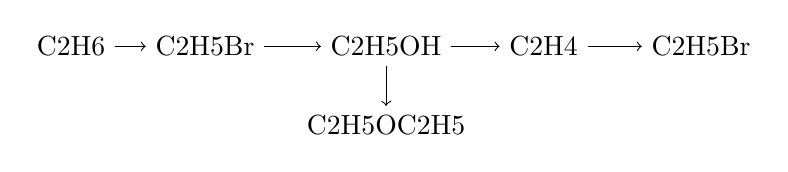
\begin{tikzpicture}
    \node(a)at (0,0) {\ce{C2H6}};
    \node(b)at (1.7,0) {\ce{C2H5Br}};
    \node(c)at (4,0) {\ce{C2H5OH}};
    \node(d)at (6,0) {\ce{C2H4}};
    \node(e)at (8,0) {\ce{C2H5Br}};
    \node(f)at (4,-1) {\ce{C2H5OC2H5}};
    \draw[->](a)--(b);
    \draw[->](b)--(c);
    \draw[->](c)--(d);
    \draw[->](d)--(e);
    \draw[->](c)--(f);
  \end{tikzpicture}\]
  \item 需要多少体积的空气（在标准状况下）才能使 \qty{23}{g} 乙醇完全燃烧？燃烧的结果能生成水和二氧化碳各多少摩尔？放出多少热量？
  \item 写出下列物质的名称，并回答它们是不是同系物？是不是同分异构体？
  \begin{tasks}(2)
    \task \ce{CH3CH2-O-CH2CH3}
    \task \ce{CH3CH2CH2CH2OH}
  \end{tasks}
  \item 某饱和一元醇 \qty{0.3}{g}，跟足量的钠起反应后，生成 \qty{56}{ml} 氢气（标准状况下），求这种一元醇的式量和化学式，并写出这种一元醇可能有的各种同分异构体的结构式和名称。
\end{question}
\end{Practice}

\section{苯酚}
跟链烃有羟基衍生物一样，芳香烃也有羟基衍生物。
在这些化合物里，羟基可以位于侧链的碳原子上，也可以直接连在苯环的碳原子上。
在芳香烃的侧链上含有羟基的衍生物叫做芳香醇，如苯甲醇（\ce{C6H5CH2OH}）。
\emph{羟基跟苯环直接相连的化合物叫做}\Concept{酚}。
苯分子里只有一个氢原子被羟基取代所得的生成物是最简单的酚，叫做苯酚，通常就简称为酚（\cref{fig:3-4}），苯酚的化学式是 \ce{C6H6O}，它的结构式是：
\[ \chemfig{HC*6(=C(-[:-90,0.5,,,draw=none]H)-CH=CH-C(-[:90]OH)=HC-[,,2])} \quad \text{简写为} \quad \chemfig{*6(=-=-(-[:90]OH)=-)} \quad \text{或} \ce{C6H5OH}\]

\begin{figure}
  \includegraphics{3-4.pdf}
  \caption{苯酚分子的比例模型}\label{fig:3-4}
\end{figure}

\subsection{苯酚的性质和用途}
\subsubsection{苯酚的物理性质}
纯净的苯酚是没有颜色的晶体，具有特殊气味，熔点是 \qty{43}{\celsius}，露置在空气里会因小部分发生氧化而显粉红色。
常温时，苯酚在水里溶解度不大，当温度高于 \qty{70}{\celsius} 时，能跟水以任意比互溶。
苯酚易溶于乙醇、乙醚等有机溶剂。
苯酚有毒，它的浓溶液对皮肤有强烈的腐蚀性，\emph{使用时要小心，如果不慎沾到皮肤上，应立即用酒精洗涤}。
焦化厂、煤气厂、化工厂、石油化工厂等的工业废水中常含酚类，如不经处理即排出，就会污染水源。
\subsubsection{苯酚的化学性质}
\paragraph{跟碱的反应——苯酚的酸性}\mbox{}\par
\begin{Experiment}
把少量苯酚晶体放入试管里，再加入 \qty{2}{ml} 水，振荡试管，由于苯酚在水里溶解度不大，溶液里出现浑浊。再逐渐滴入 5\% 的氢氧化钠溶液，继续振荡试管，可以看到溶液变为透明澄清。
\end{Experiment}
苯酚和碱反应，生成了易溶于水的苯酚钠。
\[\schemestart 
\chemfig{[:-30]*6(-=-(-OH)=-=)} \+ \ce{NaOH}
\arrow(.mid east--.mid west)
\chemfig{[:-30]*6(-=-(-ONa)=-=)} \+ \ce{H2O}
\schemestop\]

在这个反应中，苯酚显示了酸性，所以苯酚俗称石炭酸。苯酚中的 \ce{O-H} 键在水分子的作用下能够发生电离：
\[\schemestart 
\chemfig{[:-30]*6(-=-(-OH)=-=)} \+ \ce{H2O}
\arrow(.mid east--.mid west){<=>}
\chemfig{[:-30]*6(-=-(-O^{-})=-=)} \+ \ce{H3O+}
\schemestop\]

但是，苯酚的酸性极弱（电离常数 $K=\num{1.28e-10}$），在水溶液中只能电离出少量 \ce{H+}，甚至不能使指示剂变色。如果在苯酚钠的水溶液里通入二氧化碳，就会有苯酚游离出来。
\[\schemestart
\chemfig{[:-30]*6(-=-(-ONa)=-=)} \+ \ce{CO2} \+ \ce{H2O}
\arrow(.mid east--.mid west)
\chemfig{[:-30]*6(-=-(-OH)=-=)} \+ \ce{NaHCO3}
\schemestop\]

这说明苯酚的酸性比碳酸还要弱（碳酸的电离常数 $K_1=\num{4.3e-7}$）。

\begin{Reading}[补充阅读]{}
苯酚分子中羟基的氧原子含有孤对 $p$ 电子，这 $p$ 电子云可以跟苯环的大 $\pi$ 键电子云从侧面有所重叠，使氧原子上的 $p$ 电子云向苯环转移，氢氧原子之间的电子云向氧原子方向转移，羟基中氢原子较易电离，使苯酚显示一定的酸性。
\[ \chemfig{[:-30]*6(-=-(-[@{a,0.5}]@{oo}\charge{90=\:}{O}-@{h}H)=-=)}
\chemmove{\draw[-stealth]([above=3pt]oo.north)to[bend right=60]([above=2pt]a);
\draw[-stealth](h)--(oo);}
\]
\end{Reading}


\paragraph{苯环上的取代反应}\mbox{}\par
苯酚能跟卤素、硝酸、硫酸等发生苯环上的取代反应。
\begin{Experiment}
在盛有少量苯酚溶液的试管中，滴入过量的浓溴水，可以观察到很快有白色沉淀生成。
\end{Experiment}
上述实验说明，向苯酚溶液里加入溴水，既不需要加热，也不用催化剂，立即生成白色的三溴苯酚沉淀。

\[\schemestart
\chemfig{*6(=-=-(-[:90]OH)=-)} \+ \ce{3Br2} 
\arrow(.mid east--.mid west) 
\chemfig{*6(=(-[:-90]Br)-=(-[:0]Br)-(-[:90]OH)=(-[:180]Br)-)}
\ce{ v } \+ \ce{3HBr}
\schemestop\]

这个反应很灵敏，常用于苯酚的定性检验和定量测定。
\paragraph{显色反应}\mbox{}\par
\begin{Experiment}
在盛有苯酚溶液的试管中，滴入几滴 \ce{FeCl3} 溶液，振荡，溶液显紫色。
\end{Experiment}
苯酚跟 \ce{FeCl3} 溶液作用能显示紫色\footnote{苯酚跟 \ce{FeCl3} 在水溶液里起反应，生成络离子而显紫色。\[\ce{6C6H5OH + Fe^3+ -> [Fe(C6H5O)6]^3- + 6H+}\]}。利用这一反应也可以检验苯酚的存在。

\begin{Theorem}{讨论}
比较苯酚和乙醇在分子结构上和性质上有什么相同点和不同点。
\end{Theorem}

\subsubsection{苯酚的用途}
苯酚是一种重要的化工原料，可用来制造酚醛塑料（俗称电木）、合成纤维（如锦纶）、医药、染料、农药等。
粗制的苯酚可用于环境消毒。
纯净的苯酚可配成洗剂和软膏，有杀菌和止痛效用。
药皂中也掺入少量的苯酚。

\subsection{苯酚的工业制法}
过去工业上主要是从煤焦油里提取苯酚的。
随着化工生产的发展，苯酚的需要量越来越大，从煤焦油提取苯酚早已不能满足需要，目前苯酚主要是采用合成法来制取的。
合成苯酚的方法有多种，一般用苯作为原料来合成。
例如，用 \ce{FeCl3} 作催化剂，可使苯氯化制得氯苯；用 \ce{Cu} 作催化剂在高温加压下，氯苯在碱性溶液中可以水解制得苯酚。
\[\schemestart 
\chemfig{[:-30]*6(-=-=-=)} \+ \ce{Cl2} 
\arrow(.mid east--.mid west){->[\scriptsize 催化剂]}
\chemfig{[:-30]*6(-=-(-Cl)=-=)}
\+ 
\ce{HCl}
\schemestop\]
\[\schemestart 
\chemfig{[:-30]*6(-=-(-Cl)=-=)}
\+ 
\ce{H2O}
\arrow(.mid east--.mid west){->[\scriptsize 催化剂][\scriptsize 高温、加压]} 
\chemfig{[:-30]*6(-=-(-OH)=-=)}
\+ 
\ce{HCl}
\schemestop\]

\begin{Practice}[习题]
\begin{question}
  \item 在澄清的苯酚钠溶液里通入二氧化碳，溶液里变得浑浊；再加入氢氧化钠溶液，溶液又会变为澄清，为什么？写出反应的化学方程式。
  \item 从煤焦油里得到了苯酚和苯的同系物的混和物，用什么方法可以把它们分离？
  \item 怎样鉴别乙醇溶液和苯酚溶液？
  \item 某种有机物含碳 76.6\%、氢 6.38\%、氧 17.02\%，它的式量是乙烷的 3.13 倍，求它的化学式。这种有机物的水溶液加氯化铁溶液呈紫色。写出它的结构式和名称。
\end{question}
\end{Practice}

\section{醛和酮}
醛和酮是含有羰\footnote{羰音 \pinyin{tang1}}基的烃的衍生物。羰基是一个碳原子和一个氧原子以双键相连而成的一种原子团（\chemfig{-C(=[:90]O)-}）。如果羰基的碳原子连着一个氢原子，就构成 \chemfig{-C(=[:90]O)-H}，这种原子团叫做醛基。\emph{分子里由烃基跟醛基相连而构成的化合物叫做}\Concept{醛}。醛类的通式是 \chemfig{R-C(=[:90]O)-H}。

\emph{分子里由羰基跟两个烃基相连而构成的化合物，叫做}\Concept{酮}。酮分子里的羰基又可叫做酮基。酮类物质的通式是
\[ \chemfig{R-C(=[:90]O)-R'}\]

\subsection{乙醛}
\subsubsection{乙醛的物理性质}
乙醛是一种没有颜色、具有刺激性气味的液体，比水轻，沸点是 \qty{20.8}{\celsius}。乙醛易挥发，能跟水、乙醇、乙醚、氯仿等互溶。

\par\medskip\noindent
\begin{minipage}{0.6\linewidth}\parindent2em
乙醛（\cref{fig:3-5}）的化学式是 \ce{C2H4O}，它的结构式是：
\[\chemfig{H-C(-[:90]H)(-[:-90]H)-C(=[:90]O)-H}\]
简写为 \chemfig{CH_3-C(=[:90]O)-H} 或 \ce{CH3CHO}。
\end{minipage}\hfill
\begin{minipage}{0.35\linewidth}
\begin{figurehere}
  \includegraphics{3-5.pdf}
  \caption{乙醛分子的比例模型}\label{fig:3-5}
\end{figurehere}
\end{minipage}

\subsubsection{乙醛的化学性质}
乙醛分子中的醛基（\chemfig{-C(=[:90]O)-H}）官能团对乙醛的主要化学性质起决定作用。
\paragraph{加成反应}\mbox{}\par
碳氧双键能够发生加成反应，例如使乙醛蒸气跟氢气的混和物，通过热的镍催化剂时，就发生加成反应，乙醛被还原成乙醇。
\[\schemestart 
\chemfig{CH_3-C(=[:90]O)-H} \+ \ce{H2} 
\arrow(.mid east--.mid west){->[\scriptsize 催化剂][\scriptsize $\triangle$]}
\ce{CH3CH2OH}
\schemestop\chemnameinit{}\]

\begin{Reading}[补充阅读]{}
羰基上的碳氧双键跟烯烃分子里的碳碳双键一样，也是由一个 $\sigma$ 键和一个 $\pi$ 键组成，能够起加成反应。
\[\chemfig{-\charge{-90[anchor=90]={\tiny\chemdelta$+$}}{C}([2]=[@{a,0.5}]@{oo}\charge{135[anchor=-45]={\tiny\chemdelta$-$}}{O})-H}
\chemmove{\draw[-stealth]([right=4pt]a)to[bend right=45]([right=4pt]oo);}
\]

由于羰基里氧原子的电负性大，从而使碳氧双键的电子云，特别是 $\pi$ 键的电子云偏向氧原子。

当极性分子，如 \ce{HCN} 跟羰基起加成反应时，带正电的原子或基团加在氧原子上，带负电的原子或基团加在碳原子上。
\[\schemestart 
\chemfig{CH_3-C(=[:90]O)-H} \+ \ce{HCN} 
\arrow(.mid east--.mid west)
\chemfig{CH_3-C(-[:90]OH)(-[:-90]CN)-H} 
\schemestop\]
\end{Reading}

\paragraph{氧化反应}\mbox{}\par
我们早已知道，氧化—还原反应是从得氧即是氧化，失氧即是还原，开始认识的。
在有机化学的反应里，通常还可以从加氢或去氢来分析，即去氢就是氧化反应，加氢就是还原反应，所以，乙醛加氢就是乙醛被还原。
乙醛还能够被弱氧化剂所氧化。
\begin{Experiment}
在洁净的试管里加入 \qty{1}{ml} 2\% 的 \ce{AgNO3} 溶液，然后一边摇动试管，一边逐渐滴入 2\% 的稀氨水，直到最初产生的沉淀恰好溶解为止（这时得到的溶液通常叫做银氨溶液）。然后再加入 3 滴乙醛，振荡后，把试管放在热水浴里温热。不久，可以观察到试管内壁上会附着一层光亮如镜的金属银。
\end{Experiment}

在这个反应里，硝酸银跟氨水起反应，生成银氨络合物，它把乙醛氧化成乙酸，乙酸跟氨生成乙酸铵，而银氨络合物的银离子被还原成金属银，附着在试管的内壁上，形成银镜，所以，这个反应叫做\Concept{银镜反应}。
\begin{gather*}
  \ce{ Ag+ + NH3.H2O = AgOH v + NH4+ } \\
  \ce{ AgOH + 2NH3.H2O = [Ag(NH3)2]+ + OH- + 2H2O }
\end{gather*}
\begin{multline*}
    \ce{ CH3CHO + 2[Ag(NH3)2]+ + 2OH- -> \\ 
    CH3COO- + NH4+ + 2Ag v + 3NH3 + H2O}
\end{multline*}

银镜反应常用来检验醛基的存在。
工业上利用这一反应原理，把银均匀地镀在玻璃上制镜或保温瓶胆（生产上常用含有醛基的葡萄糖作为还原剂）。

乙醛也能被另一种弱氧化剂，即新制的氢氧化铜所氧化。
\begin{Experiment}
在试管里加入 10\% \ce{NaOH} 溶液 \qty{2}{ml}，滴入 2\% \ce{CuSO4} 溶液 \numrange{4}{6} 滴，振荡。然后加入乙醛溶液 \qty{0.5}{ml}，加热到沸腾。观察溶液中有红色沉淀产生。
\end{Experiment}
由于乙醛具有还原性，所以能把反应中生成的氢氧化铜还原成红色的氧化亚铜沉淀。
这也是检验醛基的一种方法。
\begin{gather*} 
  \ce{ Cu^2+ + 2OH- =Cu(OH)2 v }\\ 
  \ce{CH3CHO + 2Cu(OH)2 ->[\triangle] CH3COOH + Cu2O v +2H2O}
\end{gather*}

\subsubsection{乙醛的用途}
乙醛是有机合成工业中的重要原料，主要用来生产乙酸、丁醇等。
例如，工业上，乙醛在一定温度和催化剂条件下，被空气氧化生成乙酸。
\[\schemestart 
\ce{2CH3CHO} \+ \ce{O2} \arrow(.mid east--.mid west){->[\scriptsize 催化剂]}
\chemname{\ce{2CH3COOH}}{\footnotesize 乙酸}
\schemestop\chemnameinit{}\]

\subsubsection{乙醛的工业制法}
乙醛最早是采用乙醇氧化法制得的，这种方法需要耗用大量粮食，后来又采用了乙炔水化法。
近年来，随着石油化工的发展，又创造了乙烯氧化法制乙醛的新技术。
\paragraph{乙炔水化法}\mbox{}\par
用汞盐（如 \ce{HgSO4}）作催化剂，乙炔跟水化合，生成乙醛。
\[ \ce{ CH#CH +  H2O ->[\text{催化剂}] CH3CHO }\]

这个方法生产的乙醛纯度较高，但操作人员在生产中容易发生汞中毒。
目前正在研究以非汞催化剂代替汞催化剂，并已取得初步成效。

\paragraph{乙烯氧化法}\mbox{}\par
在一定温度和压强下，用氯化钯（\ce{PdCl2}）和氯化铜（\ce{CuCl2}） 作催化剂，使乙烯被空气或氧气直接氧化成乙醛。
\[ \ce{ 2CH2=CH2 +  O2 ->[\text{催化剂}][\text{加热、加压}] 2CH3CHO }\]

乙烯可以由石油裂化气中取得。
用乙烯氧化法生产乙醛，流程简单，原料丰富，成本低，产率高。

\subsection{醛类}
除乙醛外，还有一些在分子结构上和化学性质上都跟乙醛相似的物质，如甲醛（\ce{HCHO}）、丙醛（\ce{CH3CH2CHO}）等。
由于醛类分子里都含有醛基，所以它们的化学性质很相似。
例如，它们都能被还原为醇，被氧化为酸，都能起银镜反应等。

在醛类中，甲醛也有广泛的用途。
甲醛也叫蚁醛，是一种无色具有强烈刺激性气味的气体，易溶于水，35\%～40\% 的甲醛水溶液叫做福尔马林。
甲醛是一种重要的有机原料，应用于塑料工业（如制酚醛树脂）、合成纤维工业、制革工业等。甲醛的水溶液具有杀菌和防腐能力，是一种良好的杀菌剂。
在农业上常用稀福尔马林溶液（0.1\%～0.5\%）来浸种，给种子消毒。
福尔马林还用来浸制生物标本。

酚醛树脂是最早生产和使用的合成树脂，由于它不易燃烧并有良好的电绝缘性能，至今还用作电木（一种塑料）的原料。

酚醛树脂通常用苯酚跟甲醛起反应而制得。这个反应可简单地表示如下：
\[\schemestart
$n$\,\chemfig{*6(=-=-(-OH)=-)} \+ $n$\chemfig{HCH=[:90,,2]O} \arrow(.mid east--.mid west)
\chemfig{*6(=-=(-[:0]CH_2-[@{cl,0.4}:0])-(-OH)=(-[@{op,0.6}:180])-)}
\polymerdelim[delimiters ={[]},depth=30pt,indice =\!n]{op}{cl}
\+ $n$\,\ce{H2O}
\schemestop\]

单体间相互反应而成高分子化合物，同时还生成小分子（如水、氨等）的反应叫做\Concept{缩聚反应}。

\subsection{丙酮}
丙酮是一种没有颜色、有气味的液体，沸点是 \qty{56.2}{\celsius}，密度是 \qty{0.7899}{g/cm^3}，易挥发，易燃烧。它可跟水、乙醇及乙醚等以任意比互溶。丙酮还能够溶解脂肪、树脂和橡胶等很多有机物，它是一种重要的有机溶剂。
\par\medskip\noindent
\begin{minipage}{0.6\linewidth}\parindent2em
丙酮（\cref{fig:3-6}）的化学式是 \ce{C3H6O}，它的结构式是
\[\chemfig{CH_3-C(=[:90]O)-CH_3}\]
简写为 \ce{CH3COCH3}。
\end{minipage}\hfill
\begin{minipage}{0.35\linewidth}
\begin{figurehere}
  \includegraphics{3-6.pdf}
  \caption{丙酮分子的比例模型}\label{fig:3-6}
\end{figurehere}
\end{minipage}\par\medskip

丙酮没有还原性，不跟银氨溶液起银镜反应。在催化剂（\ce{Ni}、\ce{Co}、\ce{Pt}、\ce{Pd} 等）存在的条件下，可以跟氢气起加成反应，生成醇。

\begin{Practice}[习题]
\begin{question}
  \item 下列哪些物质可以发生银镜反应？
  \begin{tasks}(4)
    \task  甲醛
    \task  乙醇
    \task* 葡萄糖（\ce{CH2OH(CHOH)4CHO}）
  \end{tasks}
  \item 某种醛的组成是含碳 62.1\%、氢 10.3\%、氧 27.6\%，它的蒸气密度是氢气的 29 倍。写出这种醛的化学式、结构式和名称。
  \item 分别写出以石油或焦炭为原料生产乙醛的有关化学方程式。
  \item 醛和酮在分子结构上有什么相同处和不同处？在性质上有什么重要区别？如何用化学方法鉴别乙醛和丙酮？
  \item 分子里含有碳、氢、氧三种元素的烃类衍生物，已学过的有醇、醚、醛、酮等类，假定它们分子里都含有 3 个碳原子，写出各类物质的结构式，说出名称，并指出哪些互为同分异构体？
\end{question}
\end{Practice}

\section{乙酸}
乙酸（\ce{CH3COOH}）是一种重要的有机酸，它是食醋的主要成分，普通的食醋中含有 3\%～5\% 的乙酸，所以乙酸又叫醋酸。
\par\medskip\noindent
\begin{minipage}{0.6\linewidth}\parindent2em
乙酸（\cref{fig:3-7}）的化学式是 \ce{C2H4O2}，它的结构式是：\chemfig{CH_3-[,0.8]C(=[:90,0.8]O)-[,0.8]OH}，简写为 \ce{CH3COOH}。

乙酸分子里的 \chemfig{-[,0.8]C(=[:90,0.8]O)-[,0.8]OH}（或\ce{-COOH}）官能团叫做羧基，它是由羰基（\chemfig{C(-[:135,0.8])(-[:225,0.8])=O}）和羟基（\ce{-OH}）组成的。
\end{minipage}\hfill
\begin{minipage}{0.35\linewidth}
\begin{figurehere}
  \includegraphics{3-7.pdf}
  \caption{乙酸分子的比例模型}\label{fig:3-7}
\end{figurehere}
\end{minipage}

\subsection{乙酸的性质}
\subsubsection{乙酸的物理性质}
乙酸是一种有强烈刺激性气味的无色液体，沸点是 \qty{117.9}{\celsius}，熔点是 \qty{16.6}{\celsius}，当温度低于 \qty{16.6}{\celsius} 时，乙酸就凝结成象冰一样的晶体，所以无水乙酸又称冰醋酸。
乙酸易溶于水和乙醇。

\subsubsection{乙酸的化学性质}
\paragraph{酸性}\mbox{}\par
乙酸具有明显的酸性，在水溶液里能电离出氢离子。
\[ \ce{ CH3COOH <=> CH3COO- + H+ }\]

乙酸是一种弱酸，它的电离常数 $K=\num{1.75e-5}$，但比碳酸的酸性强，它具有酸的通性。

\begin{Reading}[补充阅读]{}\par\medskip\noindent
\begin{minipage}{0.75\linewidth}\parindent2em
羧基里的羰基跟醛基里的羰基相似，也是由一个 $\sigma$ 键和一个 $\pi$ 键组成，碳氧键的电子云偏向氧原子。羟基里的氧原子含有孤对 $p$ 电子，这 $p$ 电子云可以跟羰基的 $\pi$ 电子云从侧面有所重叠，使羟基氧原子的电子云向羰基转移，氢氧原子间的电子云向氧原子转移，使氢原子能够电离，具有羧基的乙酸等显示酸性。
\end{minipage}\hfill
\begin{minipage}{0.23\linewidth}
\[\chemfig{-C([2]=[@{a1,0.5}]@{o1}O)-[@{a2,0.5}]@{o2}\charge{90=\:}{O}-H}
\chemmove{\draw[-stealth]([xshift=4pt]a1)to[bend right=60]([xshift=4pt]o1);\draw[-stealth]([yshift=4pt]o2.north)to[bend right=60]([yshift=2pt]a2);}
\]
\end{minipage}
\end{Reading}

\paragraph{酯化反应}\mbox{}\par
在有浓硫酸存在并加热的条件下，乙酸能够跟乙醇发生反应，生成乙酸乙酯。
\begin{Experiment}
在试管里先加入 \qty{3}{ml} 乙醇，然后一边摇动，一边慢慢地加入 \qty{2}{ml} 浓硫酸和 \qty{2}{ml} 冰醋酸。按\cref{fig:3-8} 装置好。用酒精灯小心均匀地加热试管 \qtyrange{3}{5}{min}。产生的蒸气经导管通到饱和碳酸钠溶液的液面上。在液面上可以看到有透明的油状液体生成，并可闻到一种香味。
\tcblower
\begin{figurehere}
  \includegraphics{3-8.pdf}
  \caption{乙酸乙酯的制备}\label{fig:3-8}
\end{figurehere}
\end{Experiment}

这种有香味的无色透明油状液体就是乙酸乙酯。
由于反应生成的乙酸乙酯在同样的条件下，又能部分地发生水解反应，生成乙酸和乙醇。
所以上述反应实际上是可逆的。
\[\schemestart 
\chemfig{CH_3-C(=[:90]O)-OH}\tikz[remember picture]\coordinate(a); \+ \tikz[remember picture]\coordinate(b); \chemfig{H-^{18}O-C_2H_5}
\arrow(.mid east--.mid west){<=>[\footnotesize 浓 \ce{H2SO4}][\footnotesize $\triangle$]}
\chemfig{CH_3-C(=[:90]O)-^{18}OC_2H_5} + \ce{H2O}
\schemestop\chemnameinit{}
\tikz[overlay,remember picture]{\draw[densely dashed]([xshift=-2em,yshift=-1ex]a)rectangle([xshift=1.5em,yshift=2.5ex]b);}\]

如果用含氧的同位素 \ce{^{18}_8O} 的乙醇跟乙酸起反应时，就发现乙酸乙酯分子里含有 \ce{^{18}_8O} 原子。所以酯化反应的过程一般是：羧酸分子中的羟基跟醇分子中的氢原子结合成水，其余部分互相结合成酯。

乙酸乙酯是属于酯类化合物的一种。
\emph{酸跟醇起作用，生成酯和水的反应叫做}\Concept{酯化反应}。

\subsection{乙酸的用途}
乙酸是一种重要的有机化工原料，用途很广泛，可用于生产醋酸纤维、合成纤维（如维纶）、喷漆溶剂、增塑剂、香料、染料、医药（如阿斯匹林） 以及农药等。
\subsection{乙酸的制法}
工业上制取乙酸的方法有多种。
过去用发产法制乙酸，即用含糖类物质发酵制乙醇，乙醇经过发酵被氧化成乙醛，乙醛进一步被氧化，即制得乙酸。
食醋就是这样制取的。
目前大都采用乙烯氧化法，较新的是烷烃直接氧化法。

\subsubsection{乙烯氧化法}
乙烯氧化法生产乙酸的原理是使乙烯在有催化剂如氯化钯（\ce{PdCl2}）和氯化铜（\ce{CuCl2}）存在的条件下，跟氧发生反应，生成乙醛。
乙醛再在催化剂如醋酸锰（\ce{(CH3COO)2Mn}）的作用下，被氧化生成乙酸。
\begin{align*}
  \ce{ 2CH2=CH2 + O2 } & \ce{ ->[\text{催化剂}] 2CH3CHO }\\
  \ce{ 2CH3CHO + O2 } & \ce{ ->[\text{催化剂}] 2CH3COOH }
\end{align*}
这种方法的原料是乙烯，可以从石油加工产品中获得，因此来源很丰富。

\subsubsection{烷烃直接氧化法}
直接氧化法又叫丁烷氧化法。
这是近来发展起来的一种新的生产乙酸的方法。
这种方法的主要原料是石油炼制所产生的低沸点烷烃（主要是 \ce{C4}～\ce{C6} 馏分），这些低沸点烷烃在一定的温度、压强和催化剂（如羧酸的钴盐等）存在的条件下，被空气中的氧气直接氧化，生成乙酸。
\[ \ce{ 2CH3CH2CH2CH3 + 5O2 ->[\text{催化剂}][\text{加温、加压}] 4CH3COOH + 2H2O }\]



\begin{Practice}[习题]
\begin{question}
  \item 写出乙酸跟下列物质起反应的化学方程式：
  \begin{tasks}(3)
    \task 金属镁，
    \task 生石灰，
    \task 苛性钠溶液，
    \task 纯碱溶液，
    \task 甲醇。
  \end{tasks}
  \item 怎样用化学方法区别乙醇、乙醛和乙酸三种物质的水溶液？
  \item \qty{10}{g} 水和 \qty{40}{g} 乙酸混和配成乙酸溶液，它的密度是 \qty{1.07}{g/cm^3}，求该乙酸溶液的摩尔浓度。
  \item 用 \qty{30}{g} 乙酸和 \qty{46}{g} 乙醇反应，如果实际产率是理论产率的 85\%，可以得到多少克乙酸乙酯？
  \item 写出以水、空气和乙烯为原料制取乙酸乙酯的各步反应的化学方程式。
\end{question}
\end{Practice}


\section{羧酸}
在有机化合物里，有一大类化合物，它们跟乙酸相似，分子里都含有羧基官能团，因而它们具有跟乙酸相似的化学性质，如有酸性，能发生酯化反应等。

\begin{table}
  \caption{几种羧酸的沸点和电离常数}\label{tab:3-2}
  \begin{tblr}{colspec={X[c]X[2,r]S[table-format=6.2]c},hline{2}=0.8pt,row{1}={m,c,guard}}
    名称 & 结构简式 & 沸点（\unit{\celsius}）& $K$ \\
    甲酸   & \chemfig{H-C(=[:90]O)-OH}              & 100.7 & \num{1.77e-4} \\
    乙酸   & \chemfig{CH_3-C(=[:90]O)-OH}           & 117.9 & \num{1.75e-5} \\
    丙酸   & \chemfig{CH_3-CH_2-C(=[:90]O)-OH}      & 140.99 & \num{1.34e-5} \\
    丁酸   & \chemfig{CH_3-CH_2-CH_2-C(=[:90]O)-OH} & 163.5 & \num{1.54e-5} \\
    苯甲酸 & \chemfig{C_6H_5-C(=[:90]O)-OH}         & 249 & \num{6.46e-5} \\
  \end{tblr}
\end{table}

\cref{tab:3-2} 里各种羧酸的分子里，跟羧基直接相连的烃基不同，所以它们的性质又有所不同。

这类\emph{在分子里烃基跟羧基直接相连接的有机化合物叫做}\Concept{羧酸}。
根据羧基所连接的烃基不同，羧酸可以分为脂肪酸（如乙酸）和芳香酸 （如苯甲酸 \ce{C6H5-COOH}）。
此外也可以根据羧酸分子中含有羧基数目来分类，含有一个羧基的叫一元羧酸，如甲酸、乙酸等；含有两个羧基的叫做二元羧酸，如乙二酸（\ce{HOOC-COOH}）、己二酸（\ce{HOOC(CH2)4COOH}）等。

一元羧酸的通式为 \ce{R-COOH}。下面介绍一些重要的羧酸。

\subsection{甲酸}
甲酸（\ce{HCOOH}）俗称蚁酸。它是无色、有刺激性气味的液体，有腐蚀性，能跟水混溶。

\par\medskip\noindent
\begin{minipage}{0.7\linewidth}\parindent2em
甲酸是羧酸里最简单的一种酸。
它的结构跟其它羧酸不同，在甲酸的分子中，跟羧基相连的不是烃基，而是氢原子。
它既具有羧基的结构（虚线圆圈内为羧基），又具有醛基的结构（方框内为醛基）。
甲酸这种结构上的特殊性，使得它既表现出羧酸的性质，又表现出醛的性质。
例如，甲酸既具有酸的通性，又有还原性。
甲酸能使银氨络离子还原为金属银，而本身被氧化为二氧化碳和水。
\end{minipage}\hfill
\begin{minipage}{0.25\linewidth}
  \centering\includegraphics{3-a.pdf}
\end{minipage}
\par\medskip

甲酸在工业上主要用作还原剂、印染工业上的媒染剂、医药上的消毒剂等。

\subsection{高级脂肪酸}
在一元羧酸里，有些酸分子的烃基含有较多的碳原子，我们把烃基里含碳原子比较多的脂肪酸叫做\Concept{高级脂肪酸}。
例如硬脂酸（\ce{C17H35COOH}）、软脂酸（\ce{C15H31COOH}）和油酸 （\ce{C17H33COOH}）等都是重要的高级脂肪酸。
其中油酸的烃基里含有一个双键，而硬脂酸和软脂酸的烃基里没有不饱和键。 
硬脂酸、软脂酸属于饱和高级脂肪酸，常温下呈固态。
油酸属于不饱和高级脂肪酸，常温下呈液态。
高级脂肪酸不溶于水。
\begin{enumerate}[1.]
  \item 高级脂肪酸分子中含有羧基，所以具有羧酸的性质。如高级脂肪酸能够跟碱溶液反应而生成盐。
  \[\schemestart
  \chemname{\ce{C17H35COOH}}{\footnotesize 硬脂酸} \+ \ce{NaOH} 
  \arrow(.mid east--.mid west)
  \chemname{\ce{C17H35COONa}}{\footnotesize 硬脂酸钠} \+ \ce{H2O}
  \schemestop\chemnameinit{}\]

  我们日常使用的肥皂的主要成分就是高级脂肪酸的钠盐。
  \item 油酸分子中有一个不饱和双键，所以油酸除了能发生上述反应外，还可以跟氢气或氯气发生加成反应。例如，液态的油酸在金属镍作催化剂的条件下，跟氢气起加成反应，就能生成固态的硬脂酸。
  \[ \ce{ C17H33COOH + H2 ->[\text{催化剂}][\triangle] C17H35COOH }\]
\end{enumerate}

\subsection{苯甲酸}
苯甲酸（\ce{C6H5-COOH}）俗名安息香酸，是属于芳香酸类的有机化合物。
它是芳香酸中分子组成最简单的一种酸。
苯甲酸是一种白色针状晶体，熔点是 \qty{122.4}{\celsius}，易升华，微溶干水，易溶于乙醇、乙醚。
苯甲酸的酸性比乙酸稍强一点。
苯甲酸是有机合成的原料，除了可以制香料外，还用来制造染料、药物等。
它的钠盐可作食物的防腐剂。

\subsection{乙二酸}
乙二酸（\ce{HOOC-COOH}）俗名草酸。
它是一个最简单的二元羧酸。
草酸是没有颜色的透明晶体。
通常含有两个分子结晶水，能溶于水或乙醇。
草酸是一种重要的化工原料，可用作还原剂和用于提炼稀有金属等。

\begin{Practice}[习题]
\begin{question}
  \item 什么叫做羧酸？羧酸的官能团是什么？它具有哪些化学性质？
  \item 甲酸水溶液能不能跟碳酸钠起反应，能不能跟银氨络离子起反应？为什么？
  \item 最简单的不饱和酸是丙烯酸（\ce{CH2=CH-COOH}）。丙烯酸能起哪些反应？并写出反应的化学方程式。
  \item 甲酸俗名蚁酸。因为蚂蚁和蜂等很多昆虫的分泌液里都含有甲酸。当我们被蜂等叮咬后，涂上一点稀氨水或稀碳酸钠溶液就可以止痒止痛，这是为什么？试写出反应的化学方程式。
  \item 怎样用化学方法鉴别以下各组物质？
  \begin{tasks}[label=(\arabic*)](2)
    \task 甲醛、甲酸和乙酸，
    \task 甲醇、甲酸和丙酸。
  \end{tasks}
\end{question}
\end{Practice}

\section{酯}
我们学过，乙酸和乙醇在有浓硫酸存在的条件下，能够发生反应，生成乙酸乙酯。同样，其它的酸也可以跟醇发生类似的反应。如甲酸跟乙醇在浓硫酸存在的条件下发生反应，生成甲酸乙酯。
\[\schemestart
\chemfig{H-COOH} \+ \chemfig{HO-C_2H_5}
\arrow(.mid east--.mid west){->[\scriptsize 浓 \ce{H2SO4}]}
\chemname{\ce{HCOOC2H5}}{\footnotesize 甲酸乙酯}
\+ \ce{H2O} 
\schemestop\chemnameinit{}\]

\emph{酸跟醇起反应，生成的一类化合物叫做}\Concept{酯}。
酯的一般通式是 \ce{RCOOR$'$}。
其中 \ce{R} 和 \ce{R$'$} 可以相同，也可以不同。
酯类化合物是根据生成酯的酸和醇的名称来命名的。
例如，\ce{CH3COOC2H5} 叫乙酸乙酯，\ce{HCOOCH3} 叫甲酸甲酯。

硝酸等无机酸也能够跟醇起反应，生成的也是酯，如：
\[\schemestart
\chemfig{C_2H_5OH} \+ \chemfig{HO-NO_2}
\arrow(.mid east--.mid west)
\chemname{\ce{HC2H5-NO2}}{\footnotesize 硝酸乙酯}
\+ \ce{H2O} 
\schemestop\chemnameinit{}\]

酯类广泛地存在于自然界里。
低级酯是有芳香气味的液体，存在于各种水果和花草中。
例如，梨里含有乙酸异戊酯，苹果和香蕉里含有异戊酸异戊酯等。
酯一般比水轻，难溶于水，易溶于乙醇和乙醚等有机溶剂。
酯可用作溶剂，并用作制备饮料和糖果的果子香料。

酯的重要化学性质是能够跟水发生水解反应。

\begin{Experiment}
  在三个试管里，各加入 6 滴乙酸乙酯。再向第一个试管里加蒸馏水 \qty{5.5}{ml}。向第二个试管里加稀硫酸（$1:5$）\qty{0.5}{ml}，蒸馏水 \qty{5}{ml}。向第三个试管里加 30\% 氢氧化钠溶液 \qty{0.5}{ml}、蒸馏水 \qty{5}{ml}。振荡均匀后，把三个试管都放入 \qtyrange{70}{80}{\celsius} 的水浴里加热。几分钟后,在第三个试管里，乙酸乙酯的气味就完全消失了。第二个试管里，还剩一点乙酸乙酯的气味。而第一个试管里乙酸乙酯的气味没有多大变化。
\end{Experiment}
实验说明，在有酸和碱存在的条件下，酯类跟水发生水解反应，生成相应的酸和醇。例如，乙酸乙酯水解后生成乙酸和乙醇。
\[\schemestart
\ce{CH3COOC2H5} \+ \ce{H2O}
\arrow(.mid east--.mid west){<=>[\scriptsize 无机酸或碱]}
\ce{CH3COOH} \+ \ce{C2H5OH} 
\schemestop\chemnameinit{}\]

酯的水解反应是酯化反应的逆反应。当酯化和水解速度相等的时候，混和物中反应处于平衡状态。
\[\schemestart
\ce{RCOOH} \+ \ce{HOR$'$}
\arrow(.mid east--.mid west){<=>[\scriptsize 酯化][\scriptsize 水解]}
\ce{RCOOR$'$} \+ \ce{H2O} 
\schemestop\chemnameinit{}\]

处于平衡状态时，酯类水解的程度跟反应条件有密切关系。
当有碱存在时，碱跟水解生成的酸发生中和反应，此时水解程度就大。
\[ \ce{ ROOH + NaOH -> RCOONa + H2O }\]
当只有无机酸存在时，它只起催化作用但不能减少水解生成的酸，水解的程度就小。

在实际生产中，可以根据需要，控制一定的条件，使反应向所需要的方向进行，如可以加碱以促进酯的水解。

\begin{Practice}[习题]
\begin{question}
  \item 写出下列物质的结构简式。
  \begin{tasks}[label=(\arabic*)](4)
    \task 丁酸乙酯，
    \task 丙酸甲酯，
    \task 丁酸辛酯，
    \task 苯甲酸乙酯。
  \end{tasks}
  \item 写出甲酸跟下列物质起反应的化学方程式，并说明怎样实现这两个反应。
  \begin{tasks}[label=(\arabic*)](2)
    \task 甲醇，
    \task 乙醇。
  \end{tasks}
  \item 哪种羧酸或酯的组成是 \ce{C3H6O2}？写出它们的结构式和名称。
  \item 怎样实现下列反应？写出有关的化学方程式。
  \begin{tasks}[label=(\arabic*)]
    \task \ce{C}$\to$\ce{CaC2}$\to$\ce{C2H2}$\to$\ce{CH3CHO}$\to$\ce{CH3COOH}$\to$\ce{CH3COOC2H5}，
    \task \ce{CH3OH}$\to$\ce{HCHO}$\to$\ce{HCOOH}$\to$\ce{HCOOC2H5}。
  \end{tasks}
  \item 某有机物的蒸气密度是空气的 3.04 倍，该有机物 \qty{2.2}{g} 燃烧后得到 \qty{1.8}{g} 水及 \qty{2.24}{L}二氧化碳（标准状况下），求该有机物的化学式。如果该有机物能发生银镜反应，并能水解生成醇和酸，试确定它的结构式，并写出有关的化学方程式。
\end{question}
\end{Practice}

\section{油脂}
油脂是人类的主要食物之一，也是一种重要的工业原料。
我们日常食用的猪油、牛油、羊油、花生油、菜籽油、豆油、棉籽油等都是油脂。

在通常的温度下，油脂有呈固态的，也有呈液态的。
一般说来，呈固态的叫做脂肪，呈液态的叫做油。
因为植物油脂通常呈液态，叫做油。
动物油脂通常呈固态，叫做脂肪。
脂肪和油统称油脂。
它们在化学成分上都是高级脂肪酸跟甘油所生成的酯，所以油脂属于酯类。

\subsection{油脂的组成和结构}
油脂是由多种高级脂肪酸如硬脂酸、软脂酸或油酸等跟甘油生成的甘油酯。它们的结构可以表示如下：
\[\chemfig{R_2-C(=[:90,0.8]O)-O-CH(-[:90,1.5]CH_2-[:180]O-[:180]C(=[:90,0.8]O)-[:180]R_1)(-[:-90,1.5]CH_2-[:180]O-[:180]C(=[:90,0.8]O)-[:180]R_3)}
\]

结构式里 \ce{R1}、\ce{R2}、\ce{R3} 代表饱和烃基或不饱和烃基。
它们可以相同，也可以不相同。
如果 \ce{R1}、\ce{R2}、\ce{R3} 相同，这样的油脂称为单甘油酯。
如果 \ce{R1}、\ce{R2}、\ce{R3} 不相同，就称为混甘油酯。
天然油脂大都为混甘油酯。

形成油脂的脂肪酸的饱和程度，对油脂的熔点有着重要的影响。
由饱和的硬脂酸或软脂酸生成的甘油酯熔点较高，呈固态。
而由不饱和的油酸生成的甘油酯熔点较低，呈液态。
由于各类油脂中所含的饱和烃基和不饱和烃基的相对量不同，因此，具有不同的熔点。

\subsection{油脂的性质}
\subsubsection{物理性质}
油脂比水轻，密度在 \qtyrange{0.9}{0.95}{g/cm^3} 之间。不溶于水，易溶于汽油、乙醚、苯等多种有机溶剂中。 在工业上，根据这一性质，可用有机溶剂来提取植物种子里的油。

\subsubsection{化学性质}
由于油脂是多种高级脂肪酸的甘油酯的混和物，而高级脂肪酸中，既有饱和的，又有不饱和的。
因此油脂兼有酯类和烯烃的一些化学性质。
\paragraph{油脂的氢化}\mbox{}\par
液态油在催化剂（如 \ce{Ni}）存在下，加热、加压可以跟氢起加成反应，提高油脂的饱和程度，生成固态的油脂。
\[\schemestart 
\chemname{\chemfig{C_{17}H_{33}COO-CH(-[:90]CH_2-[:180]C_{17}H_{33}COO)(-[:-90]CH_2-[:180]C_{17}H_{33}COO)}}{\footnotesize 油酸甘油酯（油）}
\+ \ce{3H2}
\arrow(.mid east--.mid west){->[\scriptsize 催化剂][\scriptsize 加热、加压]}
\chemname{\chemfig{C_{17}H_{35}COO-CH(-[:90]CH_2-[:180]C_{17}H_{35}COO)(-[:-90]CH_2-[:180]C_{17}H_{35}COO)}}{\footnotesize 硬脂酸甘油酯（脂肪）}
\schemestop\chemnameinit{}\]

这个反应叫做油脂的氢化，也叫油脂的硬化。
这样制得的油脂叫人造脂肪，通常又叫硬化油。
工业上常利用油脂的氢化反应把多种植物油转变成硬化油。
硬化油性质稳定、不易变质、便于运输，可用作制造肥皂、脂肪酸、甘油、人造奶油等的原料。

\paragraph{油脂的水解}\mbox{}\par
跟酯类的水解反应相同，在适当的条件下（如有酸或碱或高温水蒸气存在），油脂跟水能够发生水解反应，生成甘油和相应的高级脂肪酸。
例如，硬脂酸甘油酯在有酸存在的条件下进行的水解反应，可以表示如下：
\[\schemestart 
\chemname{\chemfig{C_{17}H_{35}COO-CH(-[:90]CH_2-[:180]C_{17}H_{35}COO)(-[:-90]CH_2-[:180]C_{17}H_{35}COO)}}{\footnotesize 硬脂酸甘油酯}
\+ \ce{3H2O}
\arrow(.mid east--.mid west){<=>[\scriptsize \ce{H2SO4}][\scriptsize $\triangle$]}
\chemname{\ce{3C17H35COOH}}{\footnotesize 硬脂酸} \+ 
\chemname{\chemfig{CH(-[:90]CH_2-OH)(-[:-90]CH_2-OH)-OH}}{\footnotesize 甘油}
\schemestop\chemnameinit{}\]

工业上根据这一反应原理，可用油脂为原料来制取高级脂肪酸和甘油。

如果油脂的水解反应，是在有碱存在的条件下进行的，那么，水解生成的高级脂肪酸便跟碱反应，生成高级脂肪酸盐。
例如硬脂酸甘油酯在有氢氧化钠存在的条件下，发生水解反应，生成硬脂酸钠和甘油。
\[\schemestart
\chemname{\chemfig{C_{17}H_{35}COO-CH(-[:90]CH_2-[:180]C_{17}H_{35}COO)(-[:-90]CH_2-[:180]C_{17}H_{35}COO)}}{\footnotesize 硬脂酸甘油酯}
\+ \ce{3NaOH}
\arrow(.mid east--.mid west)
\chemname{\ce{3C17H35COONa}}{\footnotesize 硬脂酸钠} \+ 
\chemname{\chemfig{CH(-[:90]CH_2-OH)(-[:-90]CH_2-OH)-OH}}{\footnotesize 甘油}
\schemestop\chemnameinit{}\]

油脂在碱性条件下的水解反应也叫\Concept{皂化反应}。

工业上就是利用皂化反应来制造肥皂。
首先把动物性脂肪（牛脂、羊脂等）、植物油（棉籽油、豆油等）和氢氧化钠溶液按一定比放在皂化锅内，用蒸气加热，同时适当搅拌。
因为有过量的碱存在，所以油脂便发生水解反应，生成高级脂肪酸的钠盐和甘油。

反应完成后，生成的高级脂肪酸钠、甘油和水形成混和液。
高级脂肪酸钠在水里形成胶体溶液，为了使肥皂和甘油充分分离，继续加热搅拌，并向锅内慢慢加入食盐细粒。
在电解质的作用下，胶体溶液被破坏，高级脂肪酸钠从混和液中析出。
这个加入食盐使肥皂析出的过程就是盐析。
此时，停止加热和搅拌，静置一定时间，溶液便分上下两层。
上层是高级脂肪酸钠，下层是甘油和食盐的混和液。
取出上层的物质，加入填充剂（如松香和硅酸钠）等，进行压滤、干燥、成型，就制成了成品肥皂。
下层溶液经分离提纯后，便得到甘油。

油脂是一种重要的营养物质,它在完全氧化（生成 \ce{CO2} 和 \ce{H2O} 时放出的热量（约 \qty{9.4}{kCal/g}）要比碳水化合物（约 \qty{4.1}{kCal/g}）放出的热量大得多。
油脂在小肠里的酶（具有催化作用的蛋白质）的作用下，发生水解，主要生成物是脂肪酸和甘油，还有些中间产物。
肠壁能吸收脂肪酸和甘油。
在肠壁细胞里，水解生成物又重新反应生成油脂。
这种油脂经由淋巴液系统到血液里，并随血液的循环进入人体各组织里进行氧化。

\begin{Reading}{去污作用和合成洗涤剂}
  \subparagraph{肥皂的去污作用}\mbox{}\par
  普通的肥皂约含 \({70}\%\) 的高级脂肪酸的钠盐，\({30}\%\) 的水和少量的盐。
  有些肥皂内还加有填充剂、香料及染料等。
  肥皂的去污作用主要是高级脂肪酸的钠盐的作用。
  从结构上看，高级脂肪酸钠的分子可以分为两部分，一部分是极性的 \ce{-COONa} 或 \ce{-COO^-}，这一部分可溶于水，叫做亲水基。另一部分是非极性的链状的烃基 \ce{-R}，这一部分在结构上跟水的差别很大，不能溶于水，叫做憎水基。憎水基具有亲油的性质。在洗涤的过程中，污垢中的油脂跟肥皂接触后，高级脂肪酸钠分子的烃基就插入油滴内。而易溶于水的羧基部分伸在油滴外面，插入水中。这样油滴就被肥皂分子包围起来（\cref{fig:3-9}）。再经摩擦、振动，大的油滴便分散成小的油珠，最后脱离被洗的纤维织品，而分散到水中形成乳浊液，从而达到洗涤的目的。

  \begin{figurehere}
    \includegraphics{3-9.pdf}\par
    {\footnotesize
      \begin{enumerate*}[1.]
      \item 亲水基
      \item 憎水基
      \item 油污
      \item 纤维织品
    \end{enumerate*}}
    \caption{肥皂去污示意图}\label{fig:3-9}
  \end{figurehere}

  \subparagraph{合成洗涤剂}\mbox{}\par
  根据对肥皂去污原理的研究，人们认识到凡是分子的两端分别具有亲水基和憎水基的物质都有一定的去污能力。
  因此，可以利用人工合成的方法来合成具有这种结构的物质作为洗涤剂。
  这就是人们日常所用的合成洗涤剂。
  目前，常用的合成洗涤剂的主要成分是烷基苯磺酸钠或烷基磺酸钠。它们的结构式分别是 \raisebox{1ex}{\chemfig[atom sep=0.7em]{-[,1.7]R-[,1.7]*6(=-=(-[,1.7]SO_3Na)-=-)}} 和 \ce{R-SO3Na}（\cref{fig:3-10}）。其中亲水基都是极性基团 \ce{-SO3Na}，憎水基分别是非极性基团 \raisebox{1ex}{\chemfig[atom sep=0.7em]{-[,1.7]R-[,1.7]*6(=-=(-)-=-)}} 和 \ce{R-{}}。式中 \ce{R} 一般是含十个以上碳原子的烃基。
  烃基含碳原子太少时，憎水作用太弱，使得憎水基跟油的结合力不强。
  相反地，烃基含碳原子太多时，就不容易“溶”于水。
  所以烃基太大或太小都不能很好地达到去污的目的。

  \begin{figurehere}
    \includegraphics{3-10.pdf}
    \caption{合成洗涤剂分子结构示意图}\label{fig:3-10}
  \end{figurehere}

  合成洗涤剂有很强的去污能力。
  湿润、乳化的能力也很强。
  跟肥皂相比，既可以节省大量油脂，它的钙盐和镁盐又能溶于水，因而不受硬水的影响。
  所以，合成洗涤剂的发展很迅速。
\end{Reading}



\begin{Practice}[习题]
\begin{question}
  \item 脂肪和油的区别在哪里？如何把油转化为脂肪？写出反应的化学方程式。
  \item 油脂在什么情况下可以水解？水解后可以得到哪些产物？写出它们的化学方程式。
  \item 各举一例说明下列各化学反应在有机化学工业上的应用，并写出反应的化学方程式。
  \begin{tasks}[label=(\arabic*)](2)
    \task 酯化，
    \task 皂化。
  \end{tasks}
  \item 如果硬脂酸甘油酯水解时，仅有 85\% 的硬脂酸甘油酯起反应，那么要制得 \qty{5}{t} 甘油，需要多少吨硬脂酸甘油酯？
\end{question}
\end{Practice}

\section{硝基化合物}
\emph{烃分子中的氢原子被硝基}（\ce{-NO2}）\emph{取代所生成的化合物叫做}\Concept{硝基化合物}。
它们的通式为 \ce{R-NO2}。
在硝基化合物的分子中，硝基 \ce{-NO2} 直接跟碳原子相连。
这跟前面学过的硝酸乙酯不同，在硝酸乙酯（\ce{C2H5O-NO2}）的分子中，硝基 \ce{-NO2} 是通过氧原子跟碳原子相连的。
所以，不能笼统地把分子中含有 \ce{-NO2} 基团的所有化合物都叫做硝基化合物。

在硝基化合物分子中，按硝基直接相连的烃基不同，可分为脂肪族硝基化合物和芳香族硝基化合物。
其中芳香族硝基化合物较为重要。
下面我们要学习的硝基苯和三硝基甲苯就是两种重要的芳香族硝基化合物。

\subsection{硝基苯}
硝基苯（\ce{C6H5NO2}）是重要的工业原料。
工业上是利用苯在浓硝酸和浓硫酸的混和酸作用下，发生硝化反应而制得的。
\[\schemestart 
\chemfig{[:-30]*6(=-=-=-)} \+ \ce{HONO2} \arrow{->[\scriptsize 浓 \ce{H2SO4}]} \chemfig{[:-30]*6(=-=(-NO_2)-=-)} \+ \ce{H2O}
\schemestop\]

硝基苯是一种没有颜色的油状液体，不纯的显淡黄色，有苦杏仁味，比水重，难溶于水，易溶于乙醇和乙醚。
硝基苯与皮肤接触或它的蒸气被人体吸收都能引起中毒。

硝基苯能被还原成苯胺。
苯胺是染料工业的重要原料，硝基苯的重要用途就是制造苯胺。
\[\schemestart 
\ce{C6H5NO2 + 3Fe + 6HCl } \arrow(.mid east--.mid west)
\chemname{\ce{C6H5NH2}}{\footnotesize 苯胺} \+ \ce{3FeCl2 + 2H2O}
\schemestop\chemnameinit{}\]

\subsection{三硝基甲苯}
2,4,6-三硝基甲苯简称三硝基甲苯（\ce{C6H2CH3(NO2)3}），又叫梯恩梯（TNT），它的结构式是：
% \[ \chemfig{HC*6(-C(-NO_2)=CH-C=C-C=[,,2])} \]
\[\chemfig{HC*6(-C(-NO_2)=CH-C(-[:0]NO_2)=C(-[:90]CH_3)-C(-[:180]O_2N)=[,,1])}\]

三硝基甲苯是一种淡黄色针状晶体，不溶于水。
在平时比较稳定，即使受热或撞击也不易爆炸。
但是在有敏感的起爆剂如雷酸汞（\ce{Hg(ONC)2}），即雷汞等引爆的情况下，就能够发生猛烈的爆炸。
所以 TNT 是一种烈性炸药。
在国防、开矿、筑路、兴修水利等方面都有广泛用途。

三硝基甲苯是利用甲苯和硝酸、硫酸的混和酸发生硝化反应来制取的。
\[\schemestart
\chemfig{*6(-=-=(-[:90]CH_3)-=)} \+ \ce{3HONO2}
\arrow(.mid east--.mid west){->[\scriptsize 浓 \ce{H2SO4}]}
\chemfig{*6(-(-[:-90]NO_2)=-(-[:0]NO_2)=(-[:90]CH_3)-(-[:180]O_2N)=)} \+ \ce{3H2O}
\schemestop\]

\begin{Practice}[习题]
\begin{question}
  \item 硝基化合物和硝酸酯在分子结构上有什么不同？写出硝基乙烷和硝酸乙酯的结构式。
  \item 根据下列各物质的结构式，说明它们各属于哪一类化合物？并说明原因。它们可以经过哪一类反应制成？
  \begin{tasks}[label=(\arabic*)](2)
    \task \chemfig{C*6(=C(-[:-90]NO_2)-C(-[:0]H)=C(-[:0]NO_2)-C(-[:90]H)=C(-[:180]O_2N)-)(-[:180]H)}
    \task \chemfig{H-C(-[:-90]H)(-[:90]C(-[:180]H)(-[:90]C(-[:180]H)(-[:90]H)-O-NO_2)-O-NO_2)-O-NO_2}
  \end{tasks}
  \item 在实验室里，\qty{39}{g} 苯经过硝化反应后得到 \qty{55}{g} 硝基苯，试计算硝基苯的产率。
\end{question}
\end{Practice}

\section{胺\texorpdfstring{\quad}{ }酰胺}
\subsection{胺}
\emph{烃分子中的氢原子被氨基}（\ce{-NH2}）\emph{取代后，生成的化合物叫做}\Concept{胺}。
例如甲烷分子中的一个氢原子被一个氨基取代后，生成的化合物叫甲胺（\ce{CH3NH2}）。
乙烷分子中的两个氢原子被两个氨基取代后，生成的化合物叫乙二胺（\ce{H2NCH2CH2NH2}）。
苯分子中的一个氢原子被氨基取代后，生成的化合物叫苯胺（\ce{C6H5NH2}）。
甲胺、乙二胺、苯胺都属于胺类化合物。
胺类化合物一般有碱性，以下介绍苯胺。

苯胺是一种重要的胺类化合物，是合成染料（苯胺染料）、 药物（磺胺药物）等的中间体。

\subsubsection{物理性质}
苯胺是一种有特殊气味的无色油状液体，在空气中很容易氧化而成红褐色。
苯胺微溶于水，易溶于醇、醚、苯等有机溶剂里，苯胺有毒。
\subsubsection{化学性质}
\begin{enumerate}
  \item 具有弱碱性
  
  苯胺和氨结构相似，可以看作氨分子里一个氢原子被苯基所取代的生成物，因而它们在性质上也有相似的地方，即苯胺和氨都具有弱碱性（苯胺的碱性比氨还要弱）。
  这因为在苯胺分子中氨基上的氮原子上具有一对孤对电子，在水溶液中能够跟 \ce{H+} 离子形成配位键，从而增加了 \ce{OH-} 离子浓度，具有弱碱性。

  \[\ce{C6H5-{}}\electformular{N}{n}{n}{x}{d}{d}{d}{x}{d}\tikz[overlay,remember picture]\coordinate(a);\ + \ \ce{H}\:\!\electformular{O}{x}{d}{d}{d}{d}{x}{d}{d}\:\!\ce{H -> C6H5-{}}\electformular{N}{n}{n}{x}{d}{d}{d}{x}{d}\tikz[overlay,remember picture]\coordinate(b);\,\ce{H+}\ + \ \electformular{O}{x}{d}{d}{d}{d}{x}{d}{d}\:\ce{H-}
  \tikz[overlay,remember picture]{
    \node at ([xshift=-0.7em,yshift=2ex]a)[above]{\ce{H}};
    \node at ([xshift=-0.7em,yshift=-0.2ex]a)[below]{\ce{H}};
    \node at ([xshift=-0.7em,yshift=2ex]b)[above]{\ce{H}};
    \node at ([xshift=-0.7em,yshift=-0.2ex]b)[below]{\ce{H}};
  }
\]
  \begin{Experiment}
    在盛有 \qty{3}{ml} 水的试管里，加入约 \qty{0.5}{ml} 的苯胺，振荡后苯胺仍不溶解。然后逐滴加入浓盐酸，就可以看到苯胺不断溶解。等到苯胺完全溶解后，再逐滴加入浓氢氧化钠溶液，就可以看到苯胺又重新析出。
  \end{Experiment}
  从上述实验可以看出，苯胺有碱性，能跟盐酸作用生成盐，这就是盐酸苯胺。这个反应跟氨和酸反应很相似。
  \[\schemestart
  \chemname{\ce{C6H5NH2}}{\footnotesize 苯胺} \+ \ce{HCl}
  \arrow(.mid east--.mid west)
  \chemname{\ce{C6H5-NH3Cl}}{\footnotesize 盐酸苯胺}
  \schemestop\chemnameinit{}\]
  \[\ce{ NH3 + HCl \xlongequal{\quad} NH4Cl }\]

  盐酸苯胺是白色片状晶体，易溶于水，它跟碱溶液作用又重新得到苯胺。这个反应也好象铵盐跟碱反应一样。
  \begin{gather*}
    \ce{ C6H5NH3Cl + NaOH -> C6H5NH2 + NaCl + H2O } \\
    \ce{ NH4Cl + NaOH \xlongequal{\quad} NH3 + NaCl + H2O}
  \end{gather*}
  \item 苯胺放在空气中，能被空气中的氧所氧化，而使它的颜色变深。用氧化剂氧化时，生成较为复杂的混和物。主要产物决定于氧化剂及实验条件。例如用重铬酸钾作氧化剂来氧化苯胺时，生成物随着氧化程度的逐渐加深，颜色由绿变蓝，最后变成黑色。这种黑色产物叫做苯胺黑，是棉制品和皮革的良好染料。
  
  苯胺还能跟其它物质发生反应，生成多种染料。所以，苯胺是合成染料的中间体。
\end{enumerate}

\subsection{酰胺}
\emph{羧酸分子中羟基被氨基取代后而生成的化合物叫做}\Concept{酰\footnote{酰音 \pinyin{xian1}}胺}。
它们的一般通式为 \chemfig{R-C(=[:90]O)-NH_2}，其中“\chemfig{R-C(=[:90]O)-}”（或 \ce{RCO-{}}）叫做酰基。
酰胺也可以看作是氨分子中的氢原子被酰基（\ce{R-CO-{}}）取代的生成物。
常见的有甲酰胺（\ce{H-CO-NH2}）、乙酰胺（\ce{CH3-CO-NH2}）、碳酰胺 （即尿素 \ce{CO(NH2)2}）、苯甲酰胺（\ce{C6H5-CO-NH2}）等。

酰胺类化合物中，常温时除甲酰胺是液体外，其余都是晶体。
低级酰胺易溶于水。

酰胺类化合物是中性物质。
在有酸或碱存在的条件下酰胺和水共同加热煮沸，就发生水解反应，生成羧酸和氨。
\[ \ce{ RCONH2 + H2O ->[\triangle] RCOOH + NH3 -> RCOONH4 } \]

一般在水解时，都要加碱或加酸，以使水解容易进行。
如果水解时加碱，生成的酸就会变成盐，氨即逸出。
\[ \ce{ RCONH2 + NaOH ->[\triangle] RCOONa + NH3 ^ } \]

\begin{Practice}[习题]
\begin{question}
  \item 写出下列物质的结构式：
  \begin{tasks}(4)
    \task 甲酰胺，
    \task 乙酰胺，
    \task 碳酰胺，
    \task 苯甲酰胺。
  \end{tasks}
  \item 苯胺跟氨在性质上有什么相似的地方？举例说明，并写出有关的化学方程式。
  \item 写出用苯作原料制取下列物质的化学方程式，并注明反应所需的条件。
  \begin{tasks}(3)
    \task 苯磺酸，
    \task 硝基苯，
    \task 苯胺。
  \end{tasks}
  \item 有一桶苯胺重 \qty{200}{kg}，它的纯度是 99\%，制取这样一桶苯胺，需用硝基苯多少千克（硝基苯的转化率为 70\%）？
\end{question}
\end{Practice}

\begin{landscape}
\section*{内容提要}
\addcontentsline{toc}{section}{内容提要}\setcounter{subsection}{0}
烃的衍生物的重要类别和各类衍生物的重要化学性质

{\small
\begin{longtblr}[theme=plain]{
  colspec={ccccX[1,c]X[3,l]},
  rowhead=1,
  hlines={genfg},
  vlines={genfg},
  hline{1,Z}={1.5pt,genfg},
  vline{1,Z}={1.5pt},
  rows={m},
  row{1}={m,c}
}
  类别 & 通式 & 官能团 & 代表性物质 & 分子结构特点 & 主要化学性质\\
  卤代烃 & \ce{R-X} & \ce{-X}& \ce{C2H5X}& \ce{C-X} 键有极性 & 
  \begin{minipage}{6.8cm}
    \begin{tabenu}
      \item 跟 \ce{NaOH} 水溶液发生取代反应，生成醇。 
      \item 消去反应：跟强碱的醇溶液共热，脱去卤化氢，生成烯烃。
    \end{tabenu}
  \end{minipage} \\
  醇 & \ce{R-OH} & \ce{-OH} & \ce{CzH5OH} & 有 \ce{O-H} 键和 \ce{C-O} 键，有极性，\ce{-OH} 直接跟链烃基相连。& 
  \begin{minipage}{6.8cm}
    \begin{tabenu}
      \item 跟金属钠反应，生成醇钠和氢气。 
      \item 跟氢卤酸反应，生成卤代烃。
      \item 脱水反应
      \begin{tabitmz} 
        \item \qty{140}{\celsius} 分子间脱水生成乙醚。
        \item \qty{170}{\celsius} 分子内脱水生成乙烯。
      \end{tabitmz} 
      \item 氧化反应，被氧化剂氧化为乙醛。
      \item 酯化反应：跟酸反应生成酯。 
    \end{tabenu}\end{minipage}\\
  酚 & & \ce{-OH} & \chemfig{*6(=-=-(-OH)=-)} & \ce{-OH} 直接跟苯环相连。 & 
  \begin{minipage}{6.8cm}
    \begin{tabenu} 
      \item 弱酸性：跟 \ce{NaOH} 反应，生成苯酚钠和水。 
      \item 取代反应：跟浓溴水反应，生成三溴苯酚白色沉淀。
      \item 显色反应：跟铁盐（\ce{FeCl3}）反应，生成紫色物质。可以检验酚的存在。
    \end{tabenu}
  \end{minipage} \\
  醛 & \chemfig{R-C(=[:90]O)-H} & \chemfig{-C(=[:90]O)-H} & \chemfig{CH_3-C(=[:90]O)-H} & &
  \begin{minipage}{6.8cm}
    \begin{tabenu} 
      \item 加成反应：加氢（\ce{Ni} 作氧化剂）生成乙醇。
      \item 具有还原性：跟铁盐（\ce{FeCl3}）反应，生成紫色物质。可以检验酚的存在。
    \end{tabenu}
  \end{minipage} \\
  酮 & \chemfig{R-C(=[:90]O)-R'} & \chemfig{C(-[:135,0.8])(-[:225,0.8])=O} & \chemfig{CH_3-C(=[:90]O)-CH_3} & \chemfig{C(-[:135,0.8])(-[:225,0.8])=O} 双键（跟醛相似），没有跟羰基相连的氢原子 &  
  \begin{minipage}{6.8cm}
    \begin{tabenu} 
      \item 加成反应。
      \item 难以氧化，没有还原性。
    \end{tabenu}
  \end{minipage} \\
  羧酸           & \chemfig{R-C(=[:90]O)-OH} & \chemfig{-C(=[:90]O)-OH} & \chemfig{CH_3-C(=[:90]O)-OH}  & 受羰基影响，\ce{O-H} 能够电离，产生 \ce{H+}，羟基活泼性增强。 & 
  \begin{minipage}{6.8cm}
    \begin{tabenu} 
      \item 具有酸类通性。
      \item 能起酯化反应。
    \end{tabenu}
  \end{minipage} \\
  酯             & \chemfig{R-C(=[:90]O)-OR'} & & \chemfig{R-C(=[:90]O)-OC_2H_5} & 分子中酰基和 \ce{OR$'$} 之间的键容易断裂。 & 发生水解反应生成羧酸和醇。\\
  {硝基\\化合物} & \ce{R-NO2} & \ce{-NO2} & \chemfig{*6(-=-=(-[:90]NO_2)-=)} & 硝基直接跟烃基里的碳原子相连接 & 易于还原成胺。\\
  胺             & \ce{R-NH2} & \ce{-NH2} & \chemfig{*6(-=-=(-[:90]NH_2)-=)} & 氨基直接跟烃基里的碳原子相连接。&
  \begin{minipage}{6.8cm}
    \begin{tabenu}
      \item 弱碱性。 
      \item 易被氧化而变色。 
    \end{tabenu}
  \end{minipage}\\
\end{longtblr}
}
\end{landscape}

\begin{Review}
\begin{question}
  \item 试分别各用一种试剂来鉴别下列各组物质：
  \begin{tasks}(3)
    \task 乙醇和乙醚，
    \task 乙醛和丁酮，
    \task 甲醛和甲酸，
    \task 乙酸钠和苯酚钠，
    \task 苯胺和苯酚，
    \task 硝基苯和苯胺。
  \end{tasks}
  \item 有两种有机物，它们的百分组成都是含碳 40\%、氢 6.67\%、氧 53.33\%，第一种有机物的式量是 30，第二种有机物的式量比第一种大一倍，它们都能起银镜反应，试求它们的结构式和名称。
  \item 在学过的物质里，找出三种能起银镜反应的物质（必须是不同属类的有机物），写出它们的名称和结构式。并从结构上说明发生银镜反应的原因。
  \item 有两试管浑浊的水溶液，只知其中之一盛着苯酚溶液，另一试管盛着苯胺溶液。在一试管里加氢氧化钠变澄清，再加盐酸又显浑浊；在另一试管里加盐酸后变澄清，再加氢氧化钠又显浑浊。哪一试管盛苯酚，哪一试管盛苯胺？为什么？写出有关化学反应方程式。
  \item 某有机物由碳、氢、氧三种元素组成，它们的质量比为 $12:3:16$，\qty{3.1}{g} 该有机物的蒸气经过换算在 \qty{27}{\celsius}，\qty{720}{mmHg} 压强下所占的体积为 \qty{1.3}{L}，求它的化学式。如该有机物能跟酸发生酯化反应，试确定它的结构式。
\end{question}
\end{Review}